% vim:tw=72 sw=2 ft=tex
%         File: EcoAudit.tex
% Date Created: 2016 Mar 02
%  Last Change: 2016 Mar 03
%     Compiler: pdflatex
%       Author: Lamn
\documentclass[12pt,a4paper]{article}
\usepackage{amsmath, amssymb}
\usepackage[utf8]{inputenc}
\usepackage[T1]{fontenc}
\usepackage[english]{babel}
\usepackage{graphicx}
\usepackage{float}

\graphicspath{{pics/}}
\title{Life Cycle report for Coast Guard vessel \\ Aluminium vs.
Composite}

\author{Adam Lang (861110-3956) \& Andreas Fr\"oderberg (880731-7577)}

\begin{document}
\maketitle

\section{Results}

The result from the Eco Audit review can be seen below, in figure
\ref{fig:AluFootEny} we can see the contributions for the Aluminium hull
and in figure \ref{fig:CompFootEny} we can see the contributions for the
composite hull.

\begin{center}
    \begin{figure}[H]
      \centering
      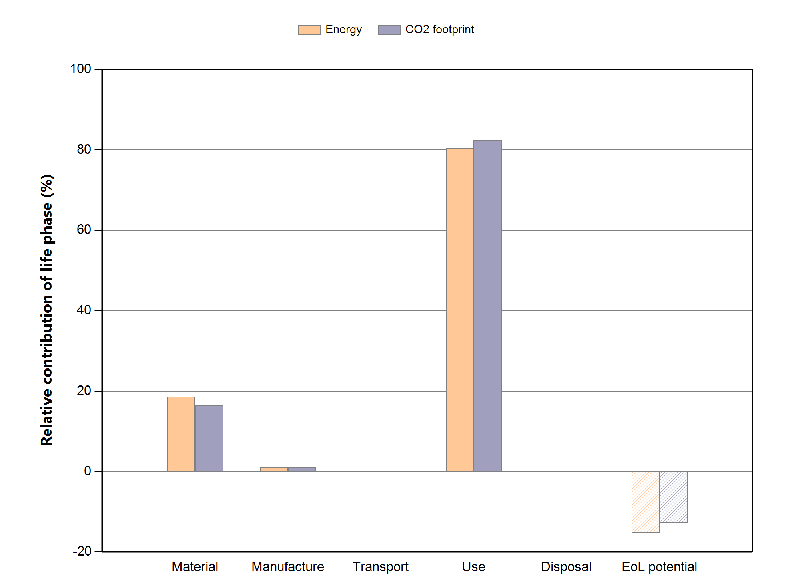
\includegraphics[scale=0.6]{AluFootEny.png}
      \label{fig:AluFootEny}
      \caption{Energy consumption and $CO_2$ footprint in the different
      faces of the products life for the Aluminium hull}
    \end{figure}
\end{center}
\begin{center}
    \begin{figure}[H]
      \centering
      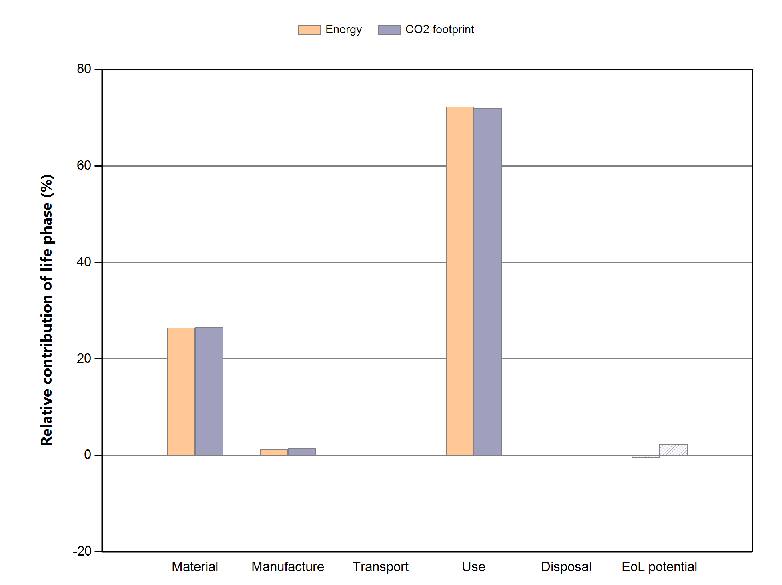
\includegraphics[scale=0.6]{CompFootEny.png}
       \caption{Energy consumption and $CO_2$ footprint in the different
      faces of the products life for the composite hull}
      \label{fig:CompFootEny}
    \end{figure}
\end{center}
Comparison between the two materials can be found in figure
\ref{fig:comp2020} and \ref{fig:comp1320}. In the figure
\ref{fig:comp2020} the both hulls have the same lifespan and in figure
\ref{fig:comp1320} the composite hull have a lifespan of 13 year and
aluminium 20 years.
\begin{center}
    \begin{figure}[H]
        \centering
        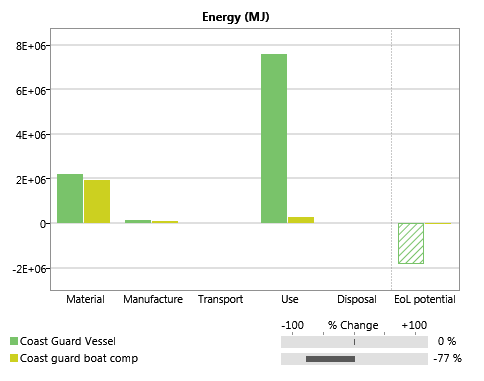
\includegraphics[scale=0.6]{comp2020.png}
        \caption{Comparison between the two materials with the same
        lifespan.}
        \label{fig:comp2020}
    \end{figure}
\end{center}

\begin{center}
    \begin{figure}[H]
      \centering
      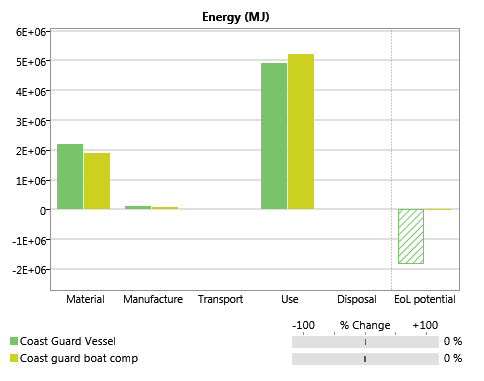
\includegraphics[scale=0.5]{comp1320.png}
      \caption{Comparison between the two materials when the composite
      have 13 years of lifespan and the aluminium has 20 years.}
      \label{fig:comp1320}
    \end{figure}
\end{center}


\section{Analysis}
  When looking at figure \ref{fig:AluFootEny} and \ref{fig:CompFootEny}
  it is clear that the largest contribution towards the $CO_2$ footprint
  and the energy consumption is during the usage phase. For the
  aluminium hull the materials production is $18.5\%$ compared to the
  usage phase contributing to $80.5\%$ of the total. This is analogue
  for the composite hull where the materials stands for about $26.4\%$
  and the usage $72.2$. For the $CO_2$ footprint we can see almost the
  same values for material, $16.5\%$ and $24.5\%$ for aluminium and
  composite respectively. The consumption and footprint during the
  manufacturing phase is negligible in comparison.

  The biggest difference between the two is that for the aluminium there
  is a recyceling possibility that is as large as $75\%$ of the
  materials consumption. This is not the case for the composite hull.

\end{document}
